\documentclass[tikz, border=3pt]{standalone}

\usepackage{amsmath,amssymb}
\usepackage{pgfplots}
\pgfplotsset{compat=1.18}
\usepgfplotslibrary{groupplots}
\usetikzlibrary{arrows.meta}
\usepackage{xcolor}

\definecolor{utnblue}{RGB}{0, 51, 102}

\pgfplotsset{
    secuencia/.style={
        axis lines=middle,
        width=9cm, height=3.6cm,
        xmin=-1.6,
        ymin=-0.35,
        xtick={-1,1,2,3,4,5,6,7},
        tick label style={font=\tiny},
        label style={font=\scriptsize},
        title style={font=\scriptsize, at={(axis description cs:1,1)},
                     anchor=north east, xshift=-2pt, yshift=-2pt},
        xticklabel style={fill=white, inner sep=1.5pt},
        every axis x label/.style={at={(ticklabel* cs:1)}, anchor=west},
        every axis y label/.style={at={(ticklabel* cs:1)}, anchor=south},
        enlargelimits=false,
        clip mode=individual,
    },
}

\begin{document}
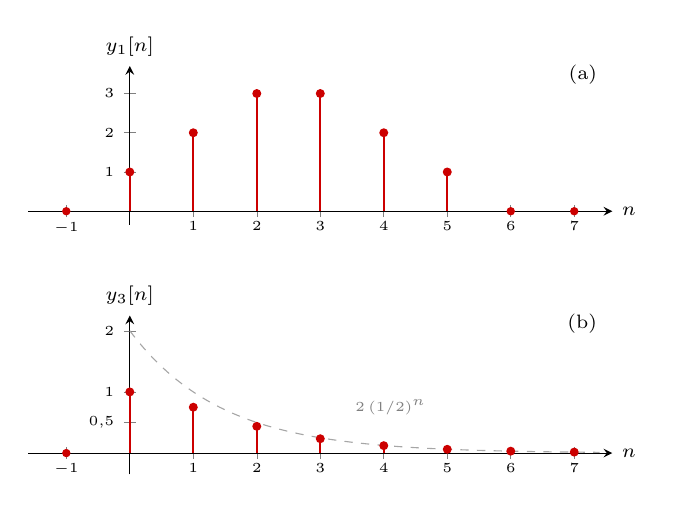
\begin{tikzpicture}[font=\scriptsize]

\begin{groupplot}[
    group style={group size=1 by 2, vertical sep=1.15cm},
    secuencia,
]

% ---------------- (a) y1[n] ----------------
\nextgroupplot[title={(a)}, ylabel={$y_1[n]$}, xlabel={$n$},
               xmax=7.6, ymax=3.7, ytick={1,2,3}]
\addplot[ycomb, red!80!black, semithick, mark=*, mark size=1.3pt,
         mark options={fill=red!80!black, draw=red!80!black}]
    coordinates {(0,1) (1,2) (2,3) (3,3) (4,2) (5,1)};
\addplot[only marks, red!80!black, mark=*, mark size=1.3pt]
    coordinates {(-1,0) (6,0) (7,0)};

% ---------------- (b) y3[n] ----------------
\nextgroupplot[title={(b)}, ylabel={$y_3[n]$}, xlabel={$n$},
               xmax=7.6, ymax=2.25, ytick={0.5,1,2},
               yticklabels={$0{,}5$, $1$, $2$}]
\addplot[dashed, gray!70, thin, mark=none, samples=100, domain=0:7.4]
    {2*(0.5)^x};
\addplot[ycomb, red!80!black, semithick, mark=*, mark size=1.3pt,
         mark options={fill=red!80!black, draw=red!80!black}]
    coordinates {(0,1) (1,0.75) (2,0.4375) (3,0.234375) (4,0.12109375)
                 (5,0.0615234) (6,0.0310059) (7,0.0155640)};
\addplot[only marks, red!80!black, mark=*, mark size=1.3pt]
    coordinates {(-1,0)};
\node[font=\tiny, gray, anchor=west] at (axis cs:3.4,0.75) {$2\,(1/2)^n$};

\end{groupplot}

\end{tikzpicture}
\end{document}
